\section{问题四：追加实验设计}

在现有 21 种催化剂组合、114 条温度实验记录的基础上，本问的目标是在新增实验总数不超过 5 次的条件下，细化高收益区域、补足关键控制变量的信息缺口，并对最终推荐条件完成一次独立复验。每次新增实验均指在确定催化剂条件和温度下，沿用原实验操作与检测规程进行一次独立性能测定。

\subsection{设计依据与总体流程}

附件 1 的记录由同一催化剂组合下的多个温度点构成，未出现的“组合--温度”单元表示尚未实验，而非缺失数值；表中为零的响应值仍是有效观测。因而，追加实验不以补值或全局黑箱外推为基础，而是围绕已有高收益温区与严格匹配结构中的实际缺格安排。附件 2 的 7 条记录属于同一次实验的不同反应时间观测，且对应催化剂编号未知，故仅用于说明独立复验中须控制测量时刻，不能将其并入任一具体催化剂组合。

图~\ref{fig:q4-flow} 给出两阶段安排。第一阶段固定执行 4 次定向实验；完成后，用新增实测结果更新两类优化任务的观测排名。第 5 次实验不继续寻找新点，而用于复验决策裕度较小任务的当前第一名，以获得推荐条件的基本重复性信息。

\begin{figure}[H]
  \centering
  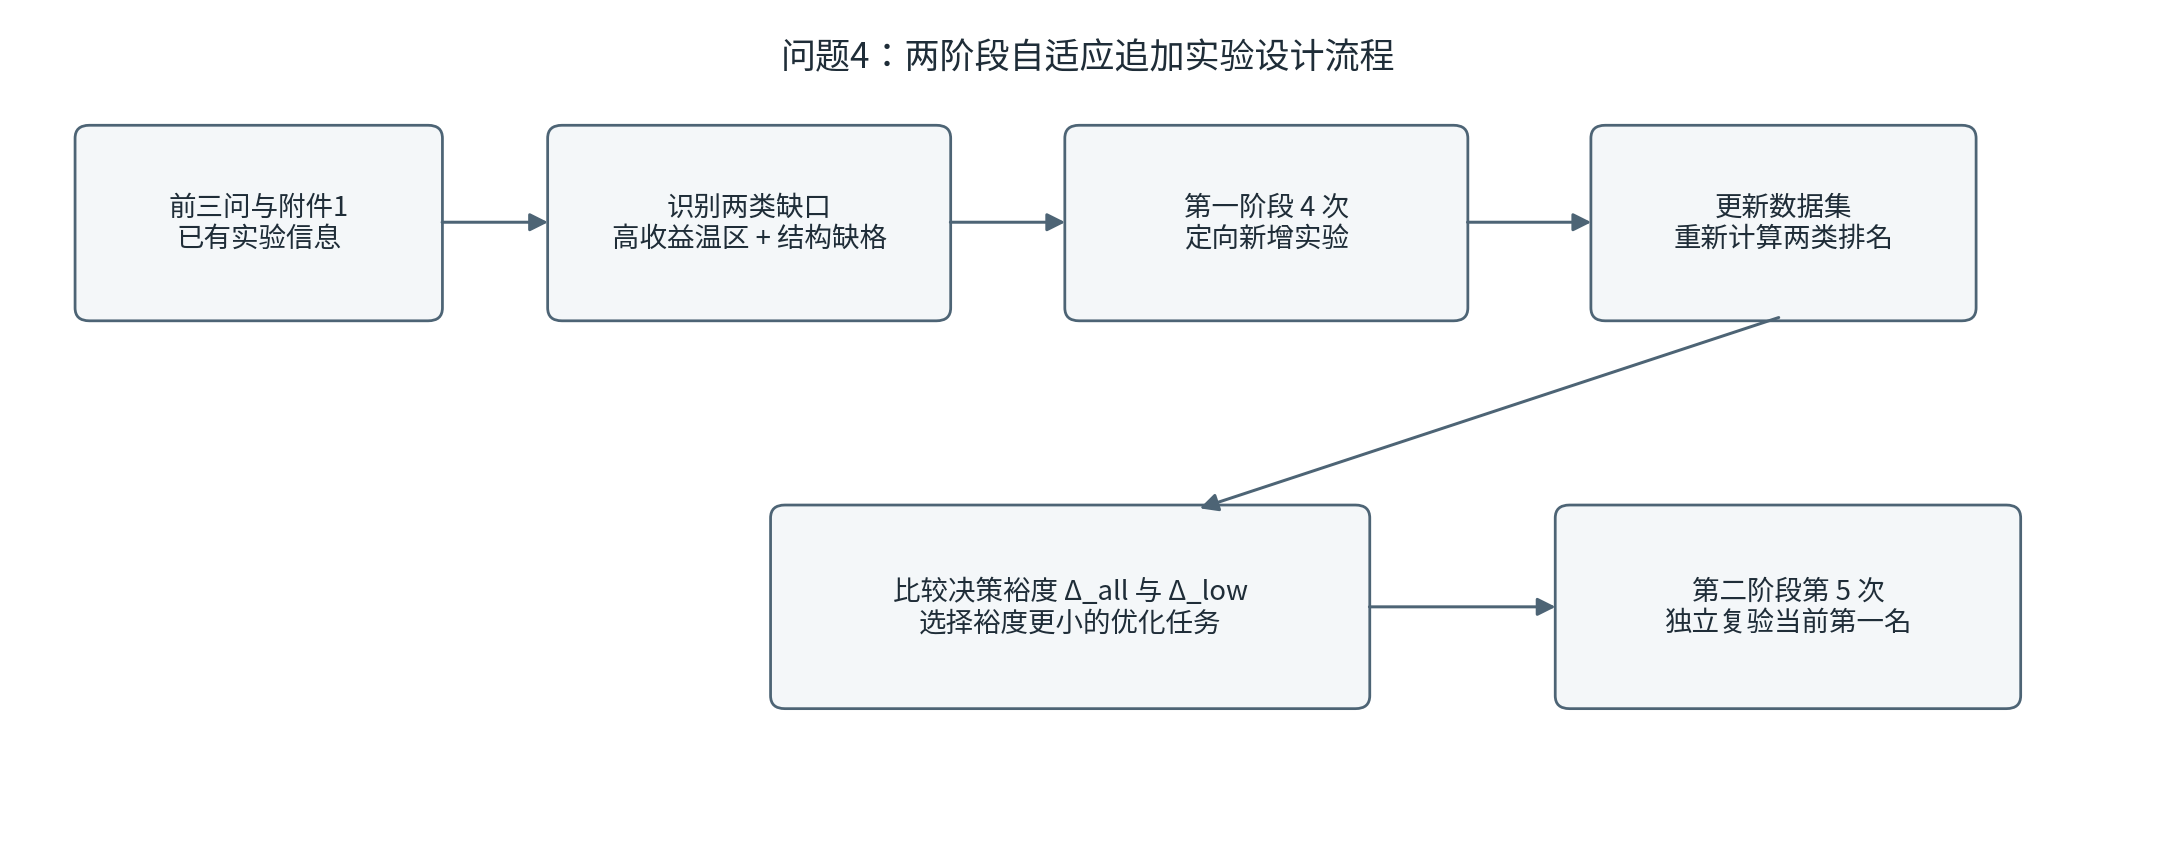
\includegraphics[width=\textwidth]{figures/q4_two_stage_experiment_design.png}
  \caption{两阶段自适应追加实验设计流程}
  \label{fig:q4-flow}
\end{figure}

对每条实测记录，仍沿用百分数尺度下的 $\mathrm{C}_4$ 烯烃收率
\begin{equation}
  Y_{\mathrm{C4}}=\frac{X_{\mathrm{EtOH}}S_{\mathrm{C4}}}{100}.
  \label{eq:q4-yield}
\end{equation}
为保持与已有结果的数值口径一致，式~\eqref{eq:q4-yield} 中的 $X_{\mathrm{EtOH}}$ 按附件表格显示精度取值。由现有观测的两类排名得到表~\ref{tab:q4-initial-rankings}：全温区的第一、第二名间隔为 1.607310 个百分点，严格 $T<\SI{350}{\degreeCelsius}$ 时的对应间隔为 6.464836 个百分点。

\begin{table}[H]
  \centering
  \caption{两类优化任务的当前观测排名与决策裕度}
  \label{tab:q4-initial-rankings}
  \small
  \begin{tabularx}{\textwidth}{L{0.17\textwidth}C{0.16\textwidth}C{0.13\textwidth}C{0.16\textwidth}C{0.13\textwidth}C{0.15\textwidth}}
    \toprule
    优化任务 & 第一名 & $Y_{(1)}$/\% & 第二名 & $Y_{(2)}$/\% & 决策裕度/百分点 \\
    \midrule
    全温区 & A3--400 ℃ & 44.720910 & A3--450 ℃ & 43.113600 & 1.607310 \\
    严格 $T<350$ ℃ & A2--325 ℃ & 17.263556 & A3--325 ℃ & 10.798720 & 6.464836 \\
    \bottomrule
  \end{tabularx}
\end{table}


\subsection{第一阶段：高收益温区与结构缺格的定向补充}

对于仅允许增加一个内部温度点的关键区间 $[a,b]$，在不预设局部响应函数形式的条件下，采用极小最大未观测温度间隔准则：
\begin{equation}
  T^{\star}=\arg\min_{a<T<b}\max\{T-a,b-T\}=\frac{a+b}{2}.
  \label{eq:q4-bisect}
\end{equation}
因此，A3 的 \SIrange{400}{450}{\degreeCelsius} 高收益区取 \SI{425}{\degreeCelsius}，A2 的 \SIrange{325}{350}{\degreeCelsius} 关键低温区取 \SI{337.5}{\degreeCelsius}。该准则只说明补点能均衡缩小温度空档，并不把补点解释为反应最优温度。

其余两次实验用于补齐严格匹配结构在 \SI{400}{\degreeCelsius} 的两个缺格。A4、A1、A2、A6 在催化材料总装料量、配比、乙醇进料条件及装料方式一致时，对应 $0.5,1,2,5$ wt\% 的 Co 负载量；其中仅 A1、A2 尚无 \SI{400}{\degreeCelsius} 记录。同时，A1/A3 和 A2/A5 分别构成仅乙醇进料条件不同的严格匹配对，且 A3、A5 已有 \SI{400}{\degreeCelsius} 记录。故 A1--\SI{400}{\degreeCelsius}、A2--\SI{400}{\degreeCelsius} 可同时补充高温 Co 负载量响应和两组进料对照信息。

\begin{table}[H]
  \centering
  \caption{第一阶段四次定向追加实验}
  \label{tab:q4-phase-one}
  \small
  \begin{tabularx}{\textwidth}{C{0.09\textwidth}C{0.18\textwidth}C{0.13\textwidth}X}
    \toprule
    实验 & 条件 & 温度 & 类型与作用 \\
    \midrule
    E1 & A3 原条件 & 425 ℃ & 组内单点二分加密，细化 400--450 ℃高收益区 \\
    E2 & A2 原条件 & 337.5 ℃ & 组内单点二分加密，细化严格低温区 325--350 ℃ \\
    E3 & A2 原条件 & 400 ℃ & 受控高温扩展；补 2 wt\% Co 高温缺格及 A2/A5 进料对照 \\
    E4 & A1 原条件 & 400 ℃ & 受控高温扩展；补 1 wt\% Co 高温缺格及 A1/A3 进料对照 \\
    \bottomrule
  \end{tabularx}
\end{table}


图~\ref{fig:q4-a3-design} 和图~\ref{fig:q4-a2-design} 分别以虚线标出两个组内补点；虚线不对应任何预设收率。图~\ref{fig:q4-co-profile} 和表~\ref{tab:q4-co-profile} 显示 \SI{400}{\degreeCelsius} 横截面中 A1、A2 的现有缺格，表~\ref{tab:q4-feed-pairs} 进一步列出两组乙醇进料严格匹配对的补全位置。

\begin{figure}[H]
  \centering
  \begin{subfigure}[b]{0.49\textwidth}
    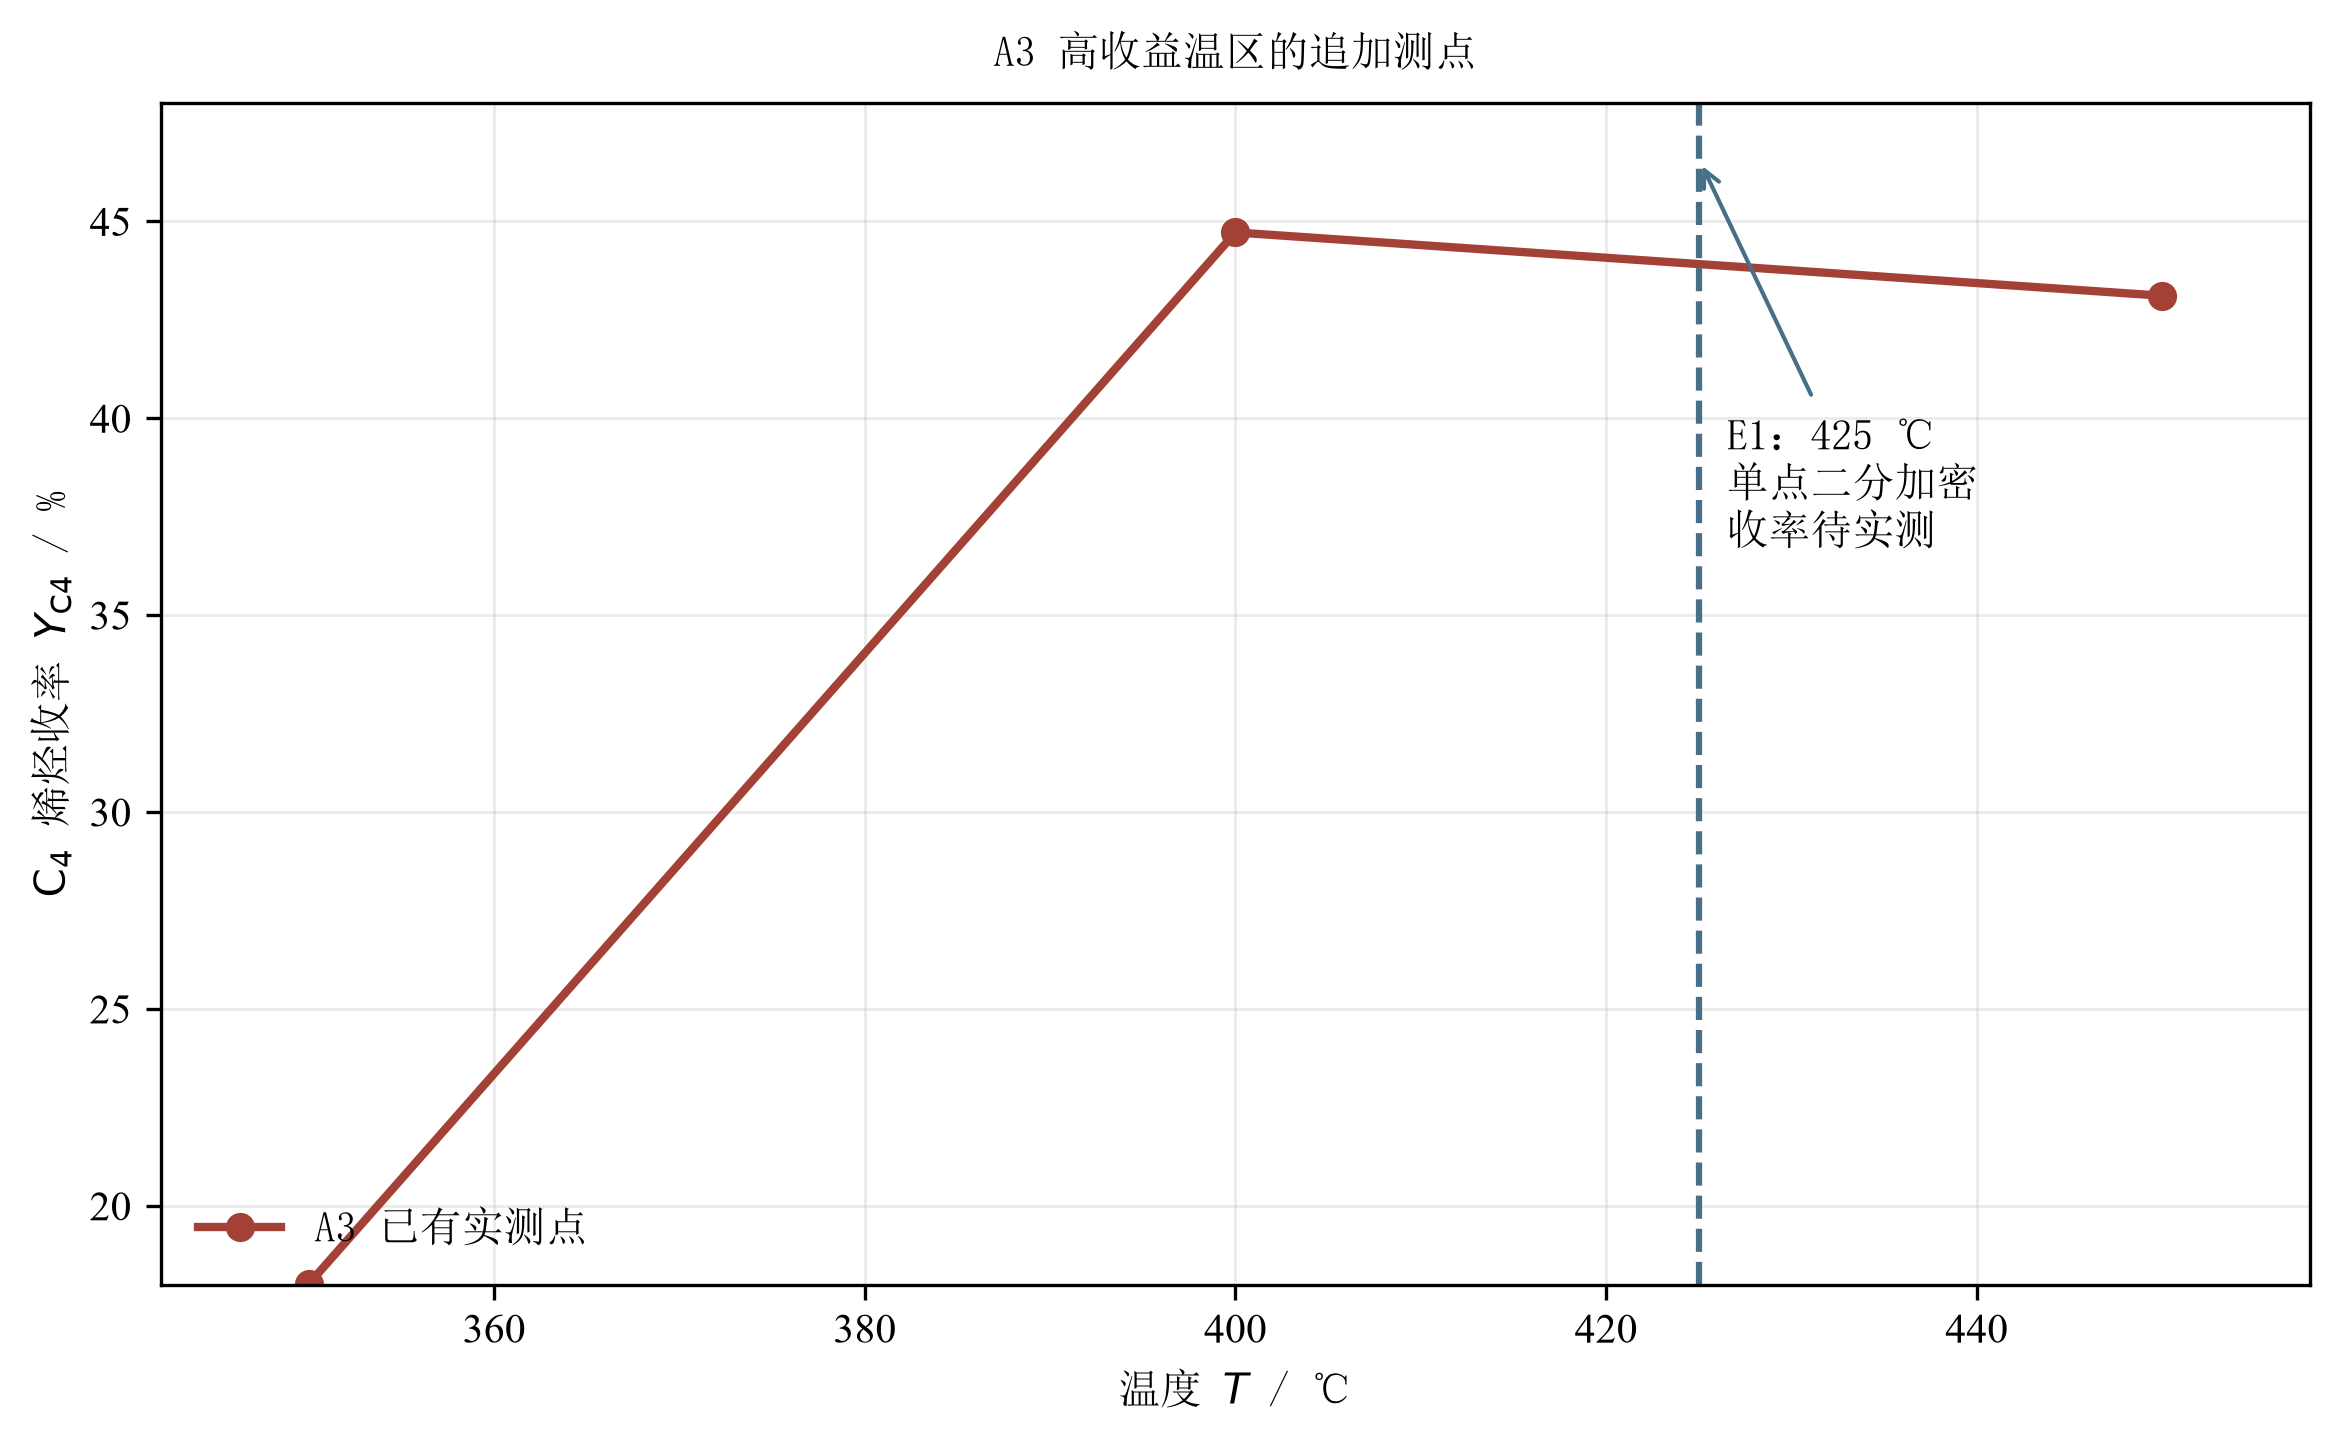
\includegraphics[width=\textwidth]{figures/q4_a3_high_temperature_design.png}
    \caption{A3 高收益温区}
    \label{fig:q4-a3-design}
  \end{subfigure}
  \begin{subfigure}[b]{0.49\textwidth}
    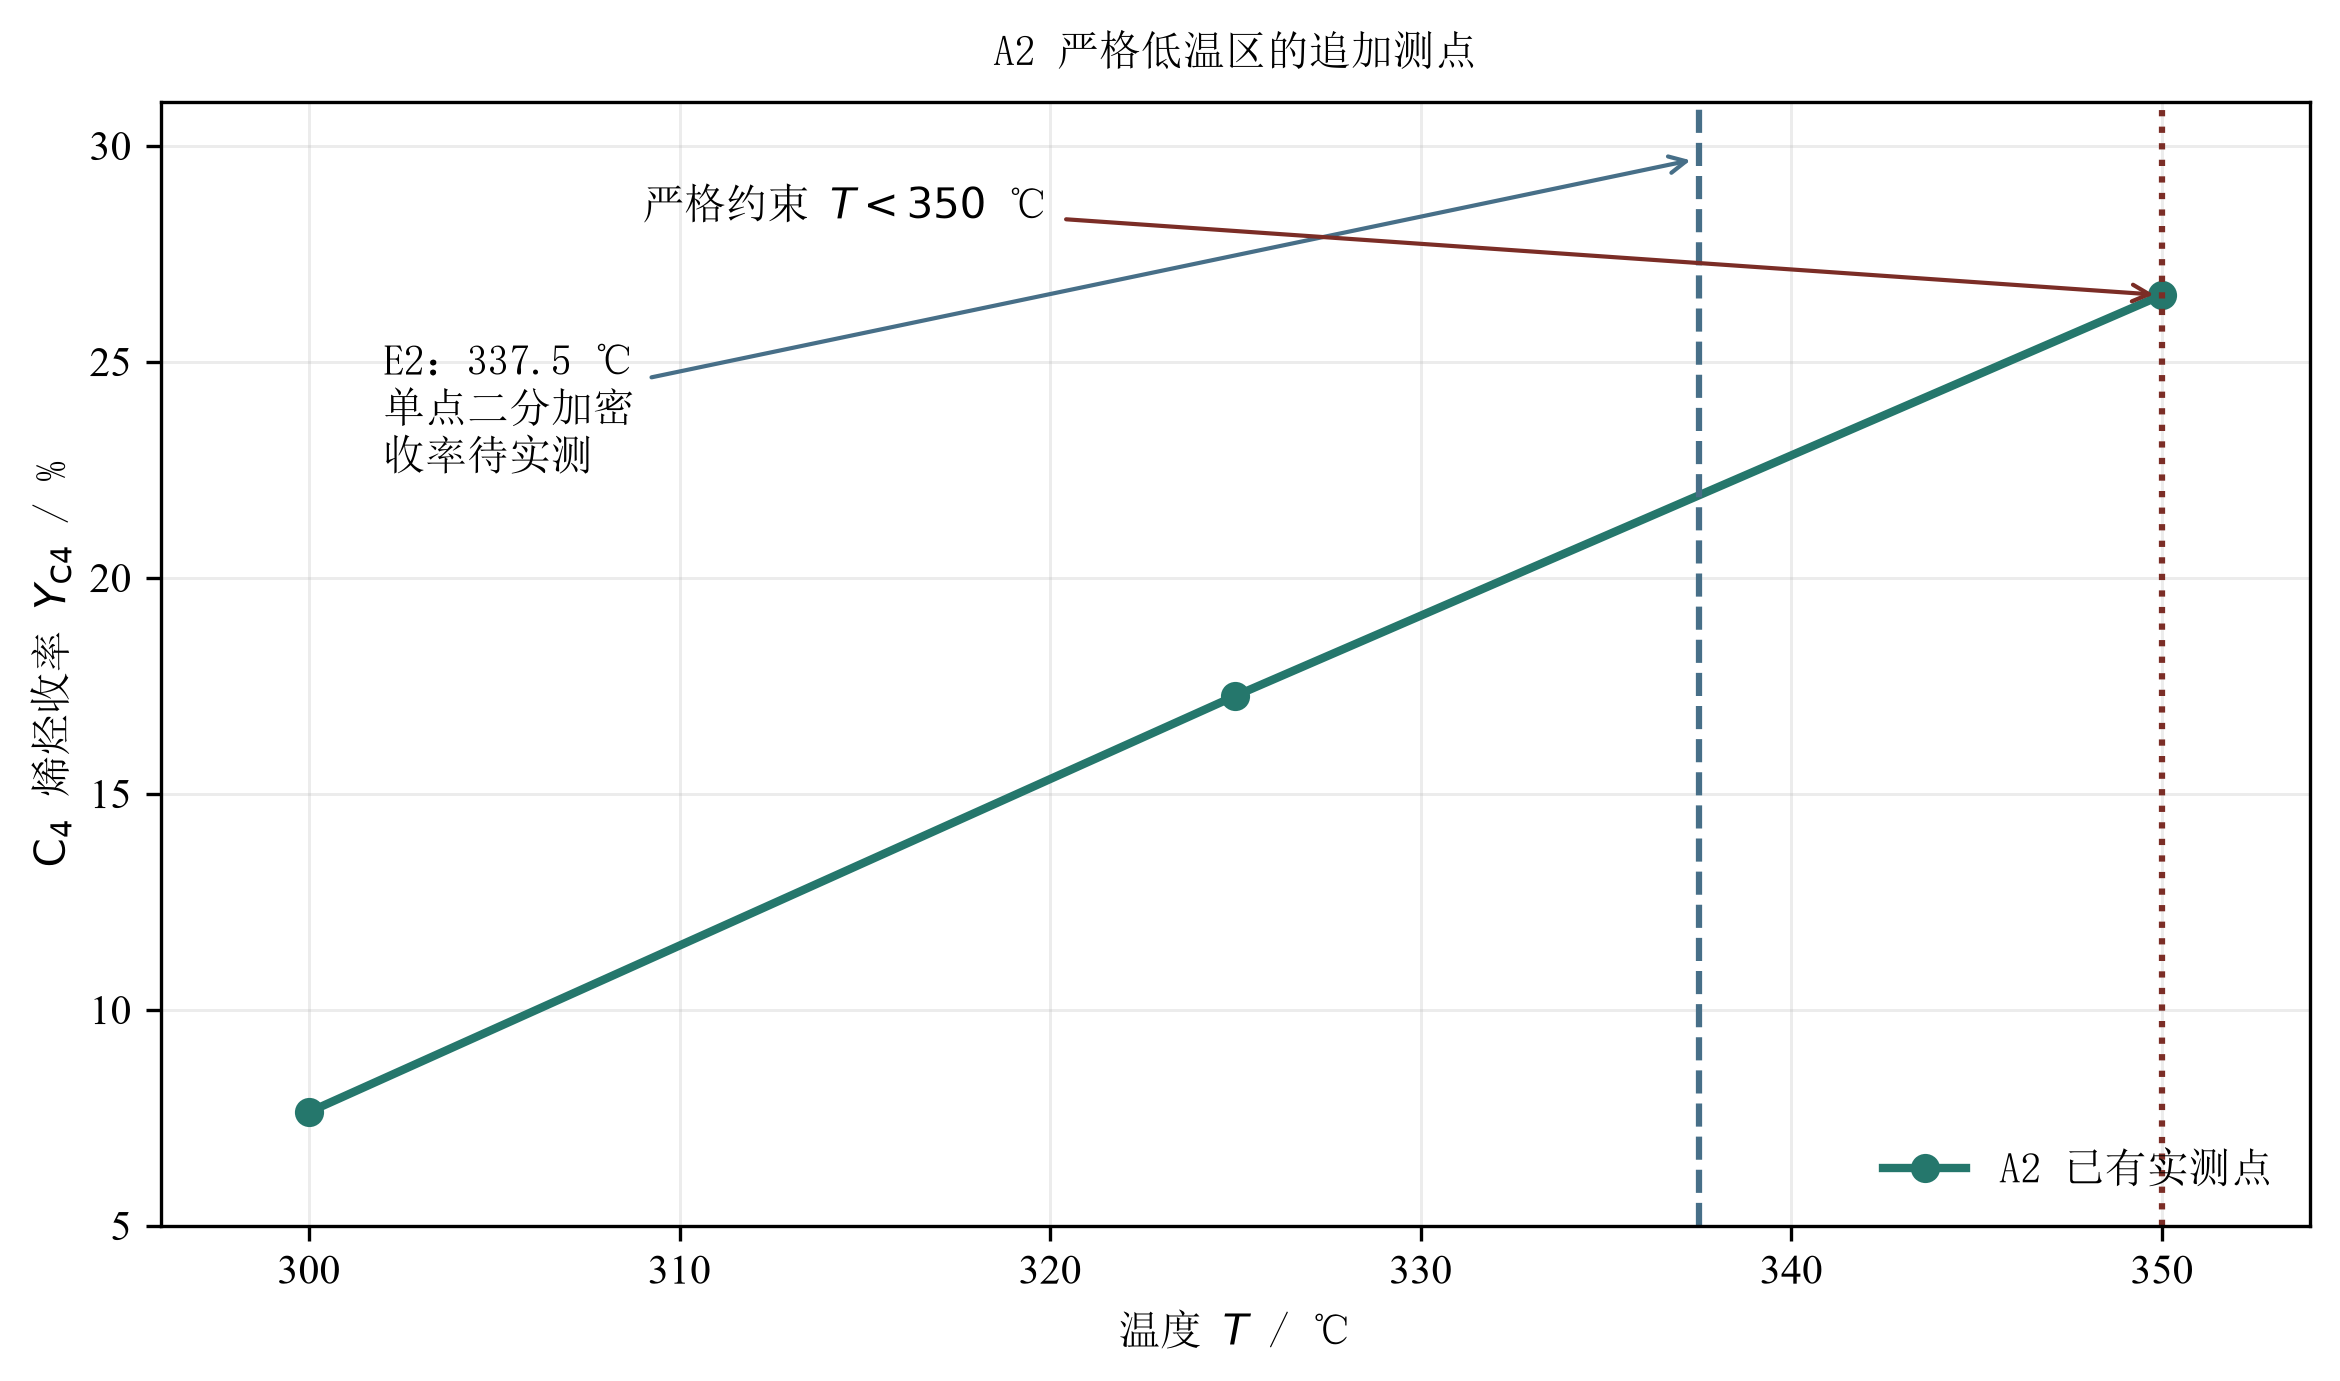
\includegraphics[width=\textwidth]{figures/q4_a2_low_temperature_design.png}
    \caption{A2 严格低温区}
    \label{fig:q4-a2-design}
  \end{subfigure}
  \caption{第一阶段的两个组内温度加密点}
\end{figure}

\begin{figure}[H]
  \centering
  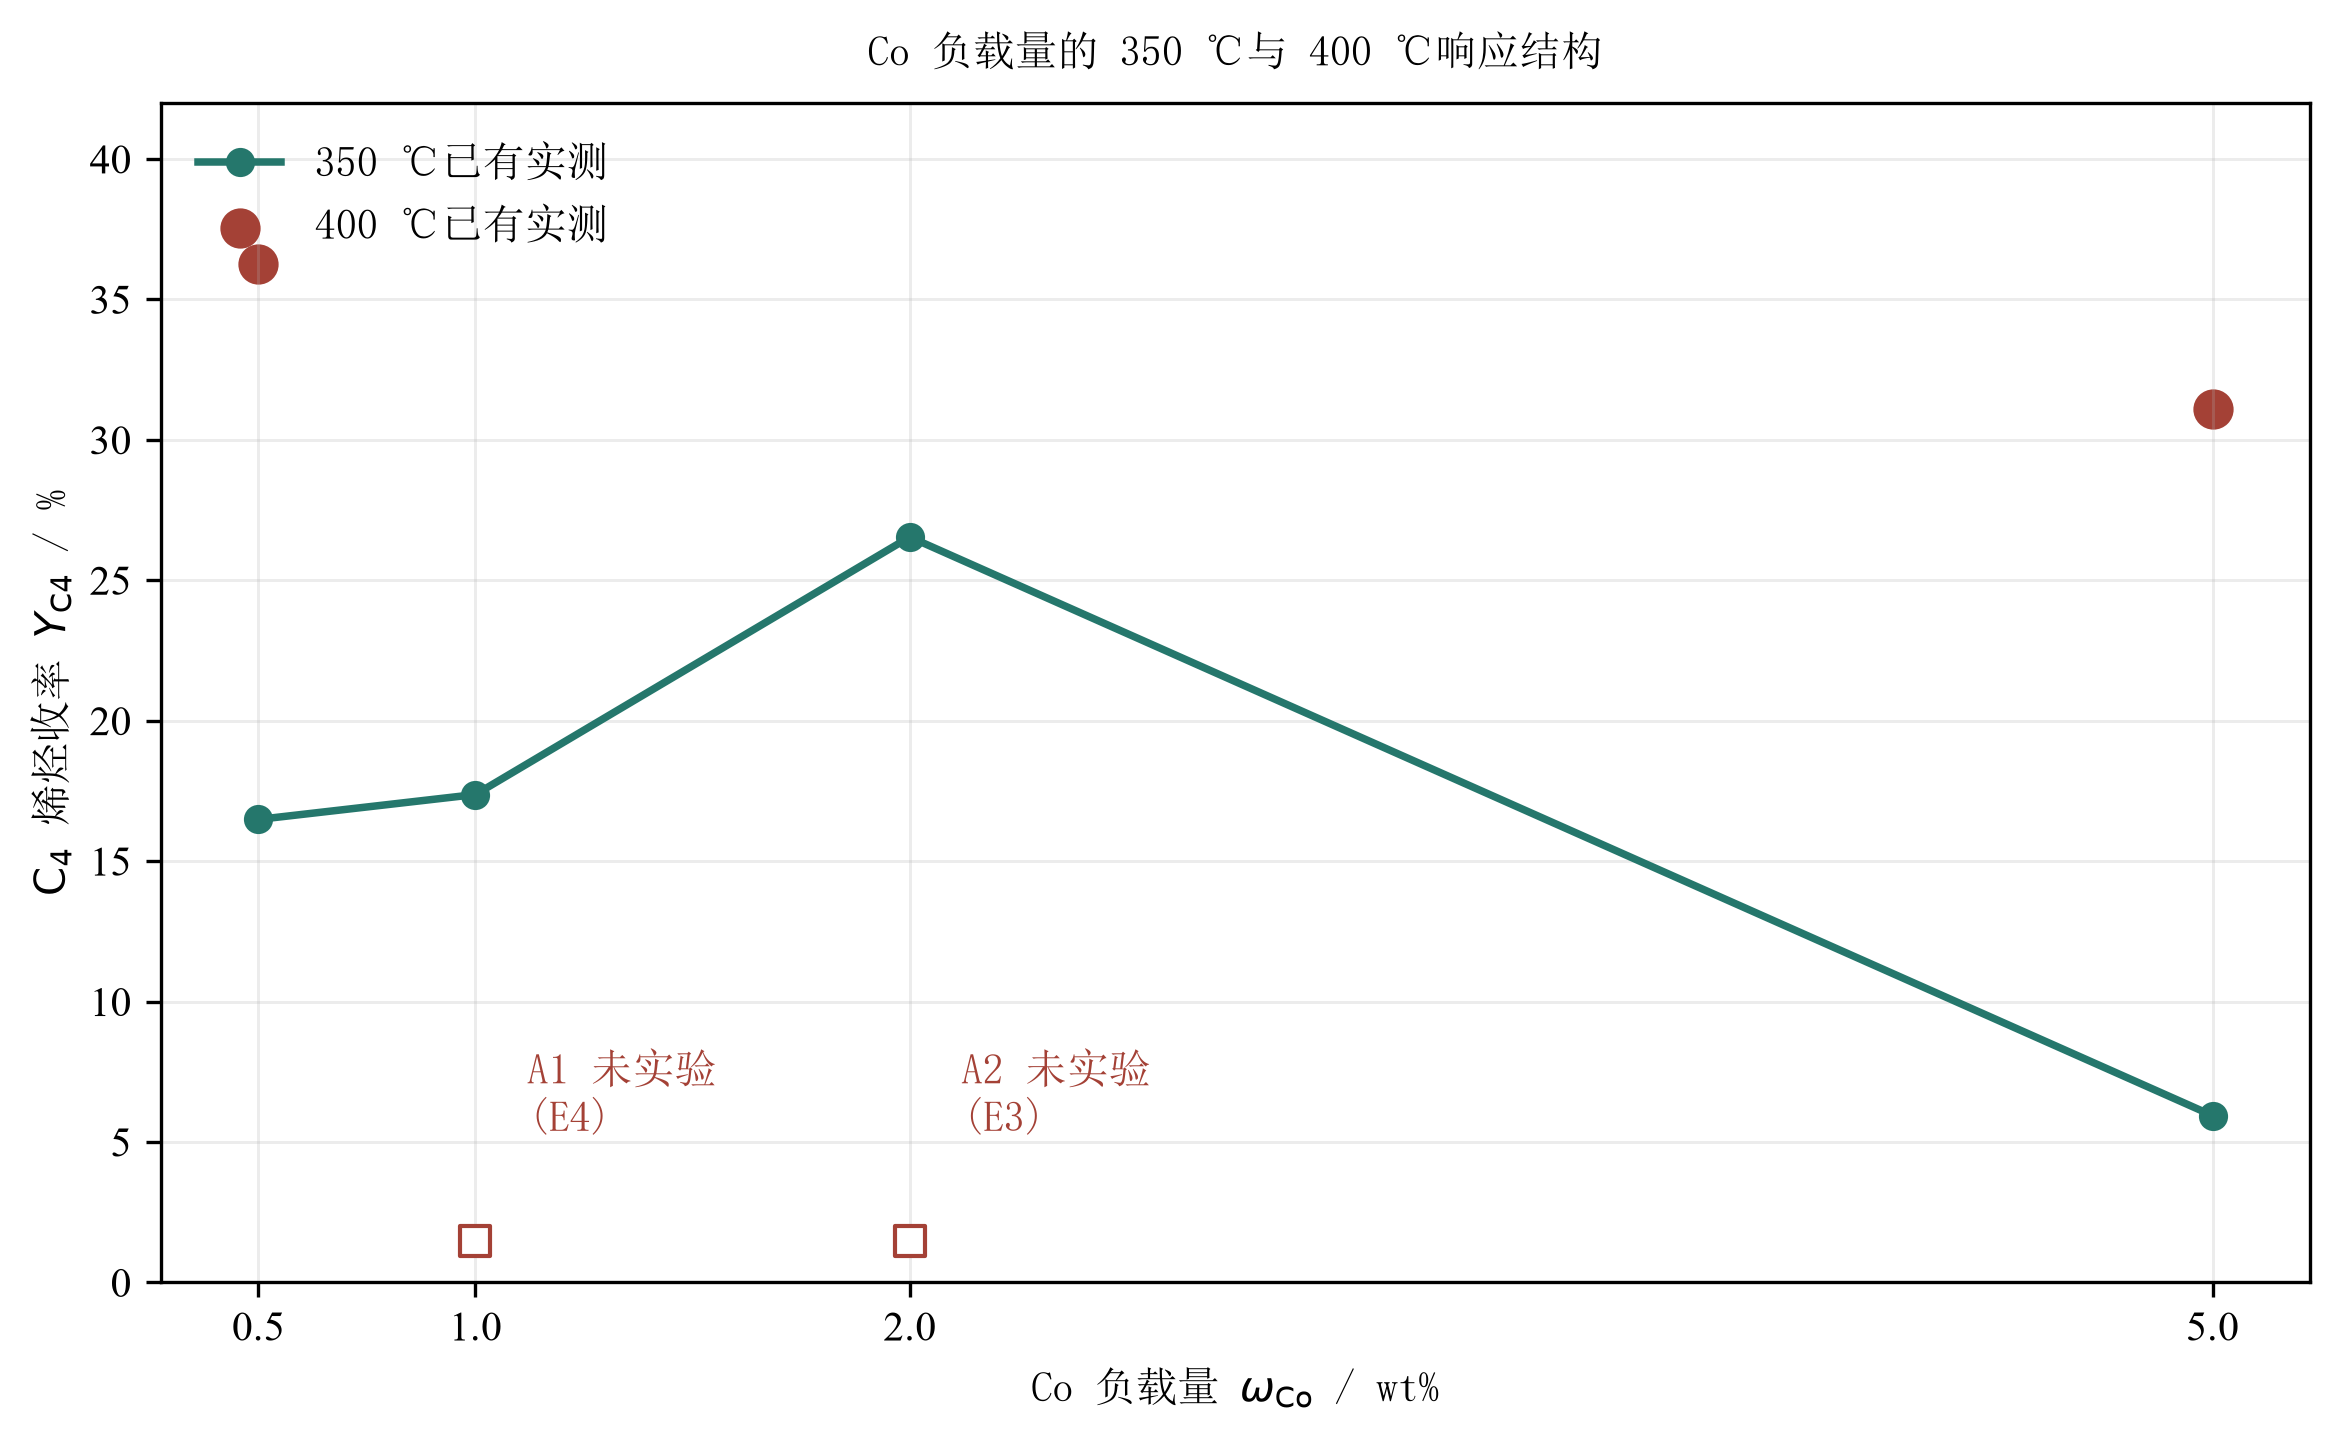
\includegraphics[width=0.84\textwidth]{figures/q4_co_loading_profile_design.png}
  \caption{Co 负载量严格匹配块在 \SI{350}{\degreeCelsius} 与 \SI{400}{\degreeCelsius} 的现有响应结构；下方空心方块表示待补的实测位置，不表示收率数值}
  \label{fig:q4-co-profile}
\end{figure}

\begin{table}[H]
  \centering
  \caption{Co 负载量严格匹配块的现有收率结构}
  \label{tab:q4-co-profile}
  \small
  \begin{tabularx}{\textwidth}{C{0.14\textwidth}C{0.18\textwidth}C{0.18\textwidth}C{0.18\textwidth}C{0.18\textwidth}}
    \toprule
    温度 & 0.5 wt\% (A4) & 1 wt\% (A1) & 2 wt\% (A2) & 5 wt\% (A6) \\
    \midrule
    350 ℃ & 16.48625 & 17.37328 & 26.54108 & 5.94270 \\
    400 ℃ & 36.26168 & 未实验 & 未实验 & 31.09589 \\
    \bottomrule
  \end{tabularx}
\end{table}

\begin{table}[H]
  \centering
  \caption{400 ℃乙醇进料严格匹配对的补全安排}
  \label{tab:q4-feed-pairs}
  \small
  \begin{tabularx}{\textwidth}{C{0.15\textwidth}C{0.17\textwidth}C{0.18\textwidth}C{0.18\textwidth}C{0.18\textwidth}}
    \toprule
    严格匹配对 & 仅改变因素 & 前者 400 ℃收率/\% & 后者 400 ℃收率/\% & 补全安排 \\
    \midrule
    A1/A3 & 乙醇进料条件 & 未实验 & 44.72091 & E4：A1--400 ℃ \\
    A2/A5 & 乙醇进料条件 & 未实验 & 29.05480 & E3：A2--400 ℃ \\
    \bottomrule
  \end{tabularx}
\end{table}


综上，第一阶段实验集合为
\begin{equation}
  \mathcal{E}_{1}=\{(\mathrm{A3},425),(\mathrm{A2},337.5),(\mathrm{A2},400),(\mathrm{A1},400)\},
  \qquad
  \mathcal{D}_{4}=\mathcal{D}_{0}\cup\mathcal{E}_{1}.
  \label{eq:q4-phase-one}
\end{equation}
其中 A3--\SI{425}{\degreeCelsius} 与 A2--\SI{337.5}{\degreeCelsius} 均位于各自已有温度范围内；A1/A2--\SI{400}{\degreeCelsius} 则属于有严格匹配结构支撑的受控高温扩展，实施前需确认设备、安全与材料可行性。若设备温控分辨率不能精确设定 \SI{337.5}{\degreeCelsius} 或 \SI{425}{\degreeCelsius}，应取最近可实现设定值，且前者仍须严格小于 \SI{350}{\degreeCelsius}。

\subsection{第二阶段：决策裕度导向的独立复验}

完成第一阶段后，分别在全温区和严格低温区内按实测收率重新确定第一、第二名，记为 $Y^{s}_{(1)}$、$Y^{s}_{(2)}$，其中 $s\in\{\mathrm{all},\mathrm{low}\}$。定义观测排名的决策裕度为
\begin{equation}
  \Delta_s=Y^{s}_{(1)}-Y^{s}_{(2)},
  \qquad
  s^{\star}=\arg\min_{s\in\{\mathrm{all},\mathrm{low}\}}\Delta_s.
  \label{eq:q4-margin}
\end{equation}
第 5 次实验 E5 对任务 $s^{\star}$ 的当前第一名进行一次新的独立实验运行。复验应保持催化剂组成、装料量、装料方式、乙醇进料条件、温度、测量时刻及操作检测规程与被复验条件一致。

在不同候选条件的实验波动量级大致可比较这一弱前提下，较小的 $\Delta_s$ 表示前两名的观测间隔更小，因而优先安排复验。该量仅作为实验排序的决策裕度，不作为显著性、置信区间或方差估计。若两类决策裕度在保留精度下相同，则应如实报告并列，结合实验安全性与实际工艺优先级确定复验对象。

若原始观测收率为 $Y_1$、独立复验收率为 $Y_2$，可报告重复均值和两次观测的样本方差：
\begin{equation}
  \overline{Y}=\frac{Y_1+Y_2}{2},
  \qquad
  s_r^2=\frac{(Y_1-Y_2)^2}{2}.
  \label{eq:q4-repeat-summary}
\end{equation}
由于仅有两次观测，上述统计量只提供基本的重复性描述；新增实验结果获得后，再据实更新两类任务的排名、E5 的复验对象及式~\eqref{eq:q4-repeat-summary} 的汇总值。

\subsection{设计边界}

本方案的 5 次预算集中用于两个高价值温度空档、两个具有严格匹配支撑的结构缺格和一次独立复验，未将同一组合的多温度记录视为大量同质独立催化剂设计，也未将 A11 作为普通 $\rho$ 配比点。由于每个新增条件初始仍只有一次观测，补齐 \SI{400}{\degreeCelsius} 横截面后只能形成完整响应剖面，不能据此进行有纯误差支持的完整双因素方差分析；一次独立复验也不足以建立可靠的总体实验误差分布。
